% Created 2015-12-20 Sun 10:30
% Indented LaTeX compiler: pdflatex
\documentclass[a5paper,openany,font 10pt]{scrbook}
\usepackage[utf8]{inputenc}
\usepackage[T1]{fontenc}
\usepackage{graphicx}
\usepackage{grffile}
\usepackage{longtable}
\usepackage{wrapfig}
\usepackage{rotating}
\usepackage[normalem]{ulem}
\usepackage{amsmath}
\usepackage{textcomp}
\usepackage{amssymb}
\usepackage{capt-of}
\usepackage{hyperref}
\makeatletter
\newcommand{\chapterauthor}[1]{%
{\parindent0pt\vspace*{-5pt}%
\linespread{1.1}\large\scshape#1%
\par\nobreak\vspace*{35pt}}
\@afterheading%
}
\makeatother
\graphicspath{{../images/cropped/}}
\date{}
\title{The Castle}
\hypersetup{
 pdfauthor={Ian Barton. Ian Barton. Ian Barton. Ian Barton.},
 pdftitle={The Castle},
 pdfkeywords={},
 pdfsubject={},
 pdfcreator={Emacs 24.5.1 (Org mode 8.3.2)},
 pdflang={English}}
\begin{document}

\maketitle
\tableofcontents

\begin{verbatim}

\end{verbatim}
NOTES:
This file sets the default LaTex options for creating the pdf file.
All the individual chapter files are INCLUDED by this file

\chapter{The Founding of the Club.}
\label{sec:orgheadline1}
\author{by Mike Anderson}
Langdale, 29th September 1967: torrential rain, the road flooded in
several places, the campsite very much the same. Hardly an auspicious
first meet for a new Club, but one that is nevertheless still
flourishing twenty one years later. All members of the Club have since
experienced similar discomforts, with the additional attractions of
cold, hail, sleet and snow. Now at last we can reveal where the
responsibility lies.

Alec Barclay came from across the Border to seek satisfaction for
causes long gone: at least that is what we put it down to when we were
induced to go to Scotland and elsewhere to be tortured by long walks
and hard climbs. Alec and his colleague Colin Mackie had first taken a
small party of Sheffielders for a weekend in Glencoe in March 1967,
followed by a further visit in July the same year. It was after these
trips that the idea of forming a club came to Alec. Discussions back
in Sheffield met with enthusiasm and convinced Alec that he had the
nucleus for the formation of a viable club.

A nine strong meeting of stalwarts held at Ashley and Avril Turner's
house on Monday 25th September 1967 led directly to the founding of
the Club. As all of them were "regulars" at The Castle Inn at Bradway
it was natural and appropriate as they intended to meet there on their
weekly club night that the Inn should lend its name to the Club. But
what to call it? The Castle Climbing Club, or The Castle
Mountaineering Club? After a long discussion it was decided to name it
"The Castle Mountaineering Club", in the belief that this title
indicating the basic principle of putting one foot in front of the
other to gain height would provide the widest possible base for the
Club and give encouragement to prospective new members.

A proposal by Alec that the Club should exist to further the spirit of
mountaineering on the one hand and to offer instruction in specific
techniques on the other, was duly accepted. It was agreed that The
Castle Inn should be the Club's headquarters until suitable premises
could be found. Alec himself would act as first Hon. Secretary and
Colin Mackie as first President, a , committee was duly elected and a
constitution adopted on 9th October 1967.

The success of The Castle Mountaineering Club owes a great deal to the
decision taken in those early days to establish the Club as a
"Mountaineering Club". Members have been encouraged over the years to
extend their mountaineering skills over a wide range of activities, be
they climbing, hill walking, skiing or pot holing even pot holing: a
little difficult to put one foot in front of the other underground and
still gain height! Whatever the activity, the Club has always afforded
opportunities for its members to acquire experience in all aspects of
climbing and mountaineering.

Regular meets were held from the outset with climbing sessions every
week on local Edges and an away meet each month to different parts of
England, Wales and Scotland. The Club rapidly became something of a
family with meetings in members' houses and with slide shows and
lectures in addition to the regular club nights at The Castle Inn.

THE FIRST STEPS HAD BEEN SUCCESSFULLY TAKEN.

But with growing membership, the need to find a clubroom which would
fulfil one of The Castle's ambitions soon became apparent. That saga,
an epic in its own right, was about to begin.


\chapter{The Clubroom Project}
\label{sec:orgheadline2}
\chapterauthor{by Mike Anderson}

It was in early July 1969, after two years of frustrating
and fruitless searching for a suitable clubroom, that Alec and
Colin were having lunch at The Rising Sun on Abbey Lane
Sheffield. Whilst discussing the Club with the licensee Ada
Bennett, they became aware of the dilapidated building behind the
Inn.

On examining the beautiful old building with its ivy covered
roof and fine stonework, it was immediately apparent that there
was great potential here in terms of the long awaited clubroom.
Interest was declared and Ada, although in favour of the
proposition, made it clear that the final decision must rest with
the Brewery and that they would need to get in touch with the
Brewery Manager.

Fortunately, our friend Mike Collins was not only the
Brewery Manager but also a "regular" at The Castle Inn where the
Club was then still meeting. He immediately took up our cause and
his enthusiasm for the project was boundless. In August 1969,
Alec had talks at The Rising Sun with a local Director of the
Brewery and members of his works department.

It was originally intended to occupy only the top half of
the building which was formerly a corn and hay loft, but on
closer inspection the upper floor joists and floor boards were
found to be riddled with woodworm and would need to be entirely
replaced: even the external doors were hanging off their hinges.
After a quick inspection the parties were glad to retire to the
more congenial surroundings of the bar of The Rising Sun to
discuss the matter further.

Now Alec had always been a talkative type of person  the
less kind might call it verbal diarrhoea  but on this occasion
this characteristic proved an invaluable asset. Alec could not or
would not stop talking, the Director needed to get back to work
and in order to get away felt obliged to promise that the Brewery
would strip out the whole of the interior of the building and
make the property structurally sound. It was agreed by Ada that
the Club could then rent the premises at a nominal figure. By the
end of September 1969, the Brewery work had been completed and
the building was available for our use.

It was at this crucial juncture that Alec presented himself
at Mike Jackson's office and asked him if he would like to be
Hon. Secretary. Mike said "No!"  Alec, it appeared, had to move
back to Scotland for business reasons and therefore unfortunately
would not be able either to continue as Hon. Secretary or take
part in the building of the clubroom. It has long been rumoured
 and believed by the very best of his friends  that Alec had
asked for a transfer back north because he had guessed what might
be in store. He asked Mike again, praising his powers of
organisation, his loyalty and the need for a steady hand on the
tiller. Mike again said "No!"   even more definitely. The verbal
diarrhoea flowed and Mike just did not stand a chance. A new Hon.
Secretary was in the making.

Our initial aspirations for the clubroom were limited to a
casual use of the existing building, although we had vague hopes
that we might be able to use one gable end as a makeshift
climbing wall. We planned to utilise our camping equipment to
provide heat and light and simply to install a few items of
second hand furniture to be donated by the Brewery. During a
visit to collect benches and stools, we noticed that the staff
were taking up the old cobbled brewery courtyard which over the
generations had been tarred in place to take the weight of horse
drawn drays. This was an opportunity too good to miss and as the
cobbles came up they were delivered to the yard of The Rising
Sun. But the mass of filthy black stone grew to alarming
proportions and it was painfully obvious that a good many
generations of horses had passed over them and left their
deposits in more ways than one.

Now the Club was fortunate in having an architect in its
ranks in the form of Kerry Brooksbank and Kerry had kindly
offered to give us a hand. On our very first day of work we
gathered in the pub yard to be greeted by a huge pile of
exceedingly evil smelling tar and horse encrusted cobbles. We
were under the impression that all we were going to do was to
clean them up as best we could and stack them into place. How
could we have been so gullible?

Looking first at the cobbles and then at us, Kerry picked
one up. It was shaped somewhat like a loaf of bread, rounded at
the top and tapered on both sides. The wearing face had been
slightly fractured by horseshoes and wagon wheels. He turned the
stone over and to our surprise, struck it sharply with his
hammer.

With a cry of "That's it!" he stood there grinning.

"That's what?" we responded in unison.

"We face it."

"We what?"

"We chisel a face on every stone."

"Every stone?"

"Every one!"

What was the man talking about? He must be joking  or had he
just taken leave of his senses? Face it? All of it? Just thinking
about it almost made us walk off and leave him standing there. He
couldn't mean it: sentenced to hard labour and rock breaking
without trial. Our hobby was mountaineering, not serving time. He
couldn't be serious\ldots{} but he was. Every single stone was to be
cut to reveal the beautiful lines and colours beneath the grime.
All twenty tons of them.

Kerry immediately undertook to prepare detailed drawings for
a stone built clubroom and then to supervise all the building
work that would be entailed, essential if the enthusiasm of
members without any building experience whatsoever was to result
in a finished product worthy of themselves and the Club. Even
then, little did we realise just what Kerry had in mind and the
magnitude of the task we were about to undertake. It was not
until he presented us with a line drawing that the full extent of
his ambitions dawned on us.

His basic plan was to convert half the ground floor of the
building into a "snug" with a room above in which to store Club
equipment. His scheme called for a raised floor for the snug room
and a massive stone centre column with embedded flagstone steps
forming a staircase to the upper floor. The inside walls were to
be stripped back to the original stonework and the ceiling of the
snug was to be of new timber supported by two substantial beams,
all the woodwork to be varnished to enhance its appearance. A
fitted bookcase would not only house books, maps and climbing
guides but also separate the snug from a small galley  bench
seating, carpets and spotlights would finish the project. ,
Having decided what to do, it only remained to do it, easier
said than done. Where were the funds, materials and labour to
come from? The last was easily solved as Club members would of
necessity have to undertake the work themselves, but financing
the project would be  more difficult with the subscription only
 1 a year. As for materials, we already had our building stone
but a great deal more material would clearly be required and so
the scrounging began.

A friendly builder gave us permission to "cannibalise" an
old bungalow about to be demolished and one evening the
equivalent of a plague of locusts descended on the unfortunate
property. Under Kerry's direction, floors and quarry tiles came
up, joists came out, many a mile of electric wire was gathered
and the lead on the roof  already being eyed by local citizens
was stripped off. The entire booty was loaded in an assortment of
vehicles and the convoy set off for home well after dark. Kerry
brought back all the lead in a borrowed Land Rover, laden to the
wheel arches. Dressed in his glad rags, covered in dust and
without any form of identification, he could hardly be expected
even to remember the registration number. It seemed to us a shame
that he was not pulled up by the local Bobby. "You won't believe
this, Officer \ldots{}"

Over the coming months many members came to lend a hand, but
the dedicated hard core were to be seen on site several evenings
a week and most weekends. The major task involved cutting the
stone, mixing cement and building the central column with its
flagstone steps. The stone was so very hard that several blows
were required to achieve even one cut on the face of each cobble
but as we gradually grew more expert it became a joy to work
with, such was its superb quality.

You could always tell our stone masons by the large painful
bruises on their hands, the strained wrists and the blood stained
finger bandages where the hammer had missed the chisel. To cover
our embarrassment, we claimed that the injuries were hand jamming
scars! We soon became adept at technical jargon and spoke
knowingly but incomprehensibly of corbels, coigns, jumpers,
gobbo, compo and lump hammers. Our world revolved around the
four to one mix. Our shoes were disgusting, our finger nails were
full of cement and our hair varied from grey to white to brown to
grey as the dust and cement flew around. -

Throughout the building programme, every single bag of sand
and cement had to be purchased and  brought on site, water was
obtained by the bucket from Ada's outhouse and lighting was by a
single lamp. When it got too dark you went home. All cement had
to be mixed by hand and all stones first cut to size and then
laid to plan. After every building session, a return visit was
required in order to brush out the mortar joints and create a
marvellous three dimensional effect.

The hundred year old ivy, previously allowed to go its own
way, covered the entire roof and gave us a different type of
problem as it was growing through the stone roof tiles and
hanging down on the inside from the ceiling to the floor. The
ancient stems were so closely entwined that the mass of
vegetation had to be laboriously cut out in small pieces, so as
not to dislodge the tiles. This was very tough work indeed and
two particularly intricate pieces were preserved in order to
display them in the clubroom fireplace.

After a daily visit over a period of several weeks to a
church under demolition, we salvaged several carved feature
stones which were sand blasted and used to support the two main
beams supplied by our friendly builder. The doors and all the
window frames were taken out and replaced, the plumbing installed
and the entire building rewired to modern standards.

Saturdays, Sundays, club nights and any spare time went into
building work and slowly, very slowly, the project began to take
shape and to resemble the plan. We felt that we were now becoming
very professional and Kerry must have thought so too, for as the
work progressed and then neared its completion, he kept coming up
with another wall to be built or a corner to be faced with stone
and even a decorative archway.

All in all it was a very busy time but like all things it
thankfully came to an end. With the snug floor laid, the centre
column built, the galley completed and the upper floor in place,
all that remained was to provide the finishing touches. Kate Peek
hand carved an archway stone dated 1970 whilst Bryan Metcalf
created a copper Castle motif with crossed ice axes to decorate
the snug fireplace. Tables, benches and chairs had been provided
by the Brewery and the carpets, together with books, maps,
pictures and photographs, were donated by members to make the
clubroom all the more comfortable and welcoming. -
The entire building programme in all its variety and
complexity was carried out by our own enthusiastic and willing
Club members, albeit under Kerry's expert guidance. The standard
achieved with little or no previous experience in building no
doubt surprised even the members themselves. Starting from
Kerry's basic concept, the carrying out of the entire project has
proved so successful that no substantial alterations have been
required over the years and the clubroom today is as fine and as
practical as ever.

However, at that time the mountaineering enthusiasts had not
fully taken into account the doubts of a number of Castle Inn
"regulars" who could not bring themselves to accept the move from
their beloved watering hole. Even after an impassioned plea from
Alec in Scotland, the move was sanctioned by the committee only
on the casting vote of the President, a remarkable performance in
the light of the magnitude of the task already undertaken and
completed.

We were now committed irrevocably to the future of the Club
and its new clubroom which we intended to use as a springboard
for our outdoor activities. But could it be viable without the
support of those early members who had stayed at The Castle Inn?
It was a question we were to ask ourselves many times over, as on
our first club night at the clubroom, a grand total of eight
turned up. Thankfully, the enthusiasm of the loyal climbing and
hill walking members prevailed and as the advantages of having
our own clubroom and meeting place became more and more apparent,
so the membership again began to grow with a welcome influx of
keen climbers and hill walkers. On 21st April 1971 a grand
opening party was held when Sir Jack Longland officially opened
the clubroom and paid tribute to the hard work and achievement of
the members.

By now we were all not only climbing and walking the hills
at every opportunity but also starting families, building careers
and setting up businesses. Nevertheless, after only a year the
stalwarts began to get itchy fingers and to prepare plans for the
erection of a climbing wall on the inside of the empty gable end
a climbing wall to give members an opportunity to fill those dark
winter nights. We learned that two cottages were being demolished
and after negotiating for the stone, we organized a number of
lorries and a further twenty tons of large sandstone blocks were
loaded and delivered to the clubroom in one day.

WE WERE OFF AGAIN!

It was a peaceful Sunday morning when the first lorry
arrived to be unloaded by members. At first the stone was neatly
stacked, but the sheer volume soon overcame our efforts. The pile
grew higher and higher until it topped the boundary wall, itself
seven feet high, by some three feet. But the fully laden lorries
kept arriving.

At the height of this activity, Ada  who had in fairness to
the Hon. Secretary had been warned that "a few stones" might be
arriving  sallied forth to express her heartfelt indignation. As
she came into the yard, a very large lorry was noisily attempting
to extricate itself from the huge mass of stone in front and the
ever growing pile it was tipping behind. The  din and the clouds
of diesel fumes were absolutely appalling. The Hon. Secretary
 remember, he's the one who got talked into this job  looked
round for moral support from the loyal members busily working at
his side. He needn't have bothered: not one was to be seen and
Ada's considerable wrath descended on him unabated and at great
length. Mike is not very often lost for words but it would have
been easier for him to dam the Grand Canyon than to put up any
resistance. He listened, tried to look intelligent and said very
little, a ploy he had already tried out unsuccessfully on Alec.
Guilty as charged!

The stone masons were brought out of their happy retirement
and the building work began again. The climbing wall progressed
quickly, as it proved much easier working indoors with power and
water laid on.  Great attention was given to detail, with
undercut holds, hand jamming cracks and overhangs constructed to
the precise requirements of the climbers. The design incorporated
an open fireplace with a flue inside the wall, mischievously
described as the one and only centrally heated climbing wall! The
fireplace itself also serves to provide a genuine mantle shelf
start to the main face.

One last area remaining for improvement was the main
entrance. A canopy was built, stone flags laid and a stone
grinding wheel erected to provide a decorative finishing touch
with local interest, this being of course The Peak District ,
 National Park emblem. Kate, as artistic as ever, carved out a
second stone, this time dated 1972.

APRIL 26TH 1972   FINISHED!

No more stone to cut, no more fittings to fit, no more
mixing of cement and no more painting. Party time with a firkin
of ale, a whole range of goodies made by wives and girlfriends, a
time to celebrate. Sir Jack Longland came back to do the honours
and we were joined in our celebrations by representatives of the
Brewery, members of other climbing clubs, the Press and all who
had made our clubroom possible. The night was long and one to
remember.

Since then, members have been involved in the promotion of a
film in Sheffield depicting the local climbing scene and the
premiere of "Whillans on Everest" in 1971, a scoop for the Club
and, even if something of a gamble, a means of meeting our
building costs. They have taken an active part in the formation
of the Sheffield Association of Climbing Clubs  SACC  and have
extended a helping hand to many, including the hard lads from
London's East End who met their match on the local gritstone
Edges. Most of all it has been fun and our clubroom provides
unique and welcoming surroundings in which the members and their
friends can enjoy each other's company and plan their outdoor
activities.

Throughout the years, the Club has certainly seen many
changes in climbing techniques, from the early days when we filed
the threads out of nuts, to the high tech "Friends" of today. It
is not unusual these days to see a pair of bright pink tights on
the climbing wall on a club night, enhancing the style of their
proud owner. Progress, it would appear, comes in many forms. Even
the Club's newsletter is computerised: now there's progress!

Members can be found visiting all parts of the world ranging
from the Himalaya to the Antarctic, from South America to Africa
and from the Rockies to the Alps   a far cry from those early
days when each away meet was an adventure in itself and a meet in
Scotland the limit of our ambitions. With Alec starting a second
Castle Mountaineering Club in Edinburgh   yes, he's at it again!
  it only remains for Kerry  who moved to Johannesburg  and for
Kate and Alan  who moved to Norway  to do the same and we shall
truly enjoy worldwide connections. ,
Throughout the first twenty one years of its existence the
Castle has enjoyed the services of outstanding Club Officers who
have taken a full and active part in organising meets and
encouraging members new and old, ensuring the smooth running and
progress of the Club. The friendship and companionship of The
Castle Mountaineering Club are very special and just as members
have given their best efforts to the Club, so the Club has
brought together many people from different walks of life to
share the joys of climbing the crags and tackling the mountains.

The foundations of The Castle Mountaineering Club have been
well laid and with its unique features and the enthusiasm of its
members, its future is clearly secure.

\begin{figure}[htb]
\centering
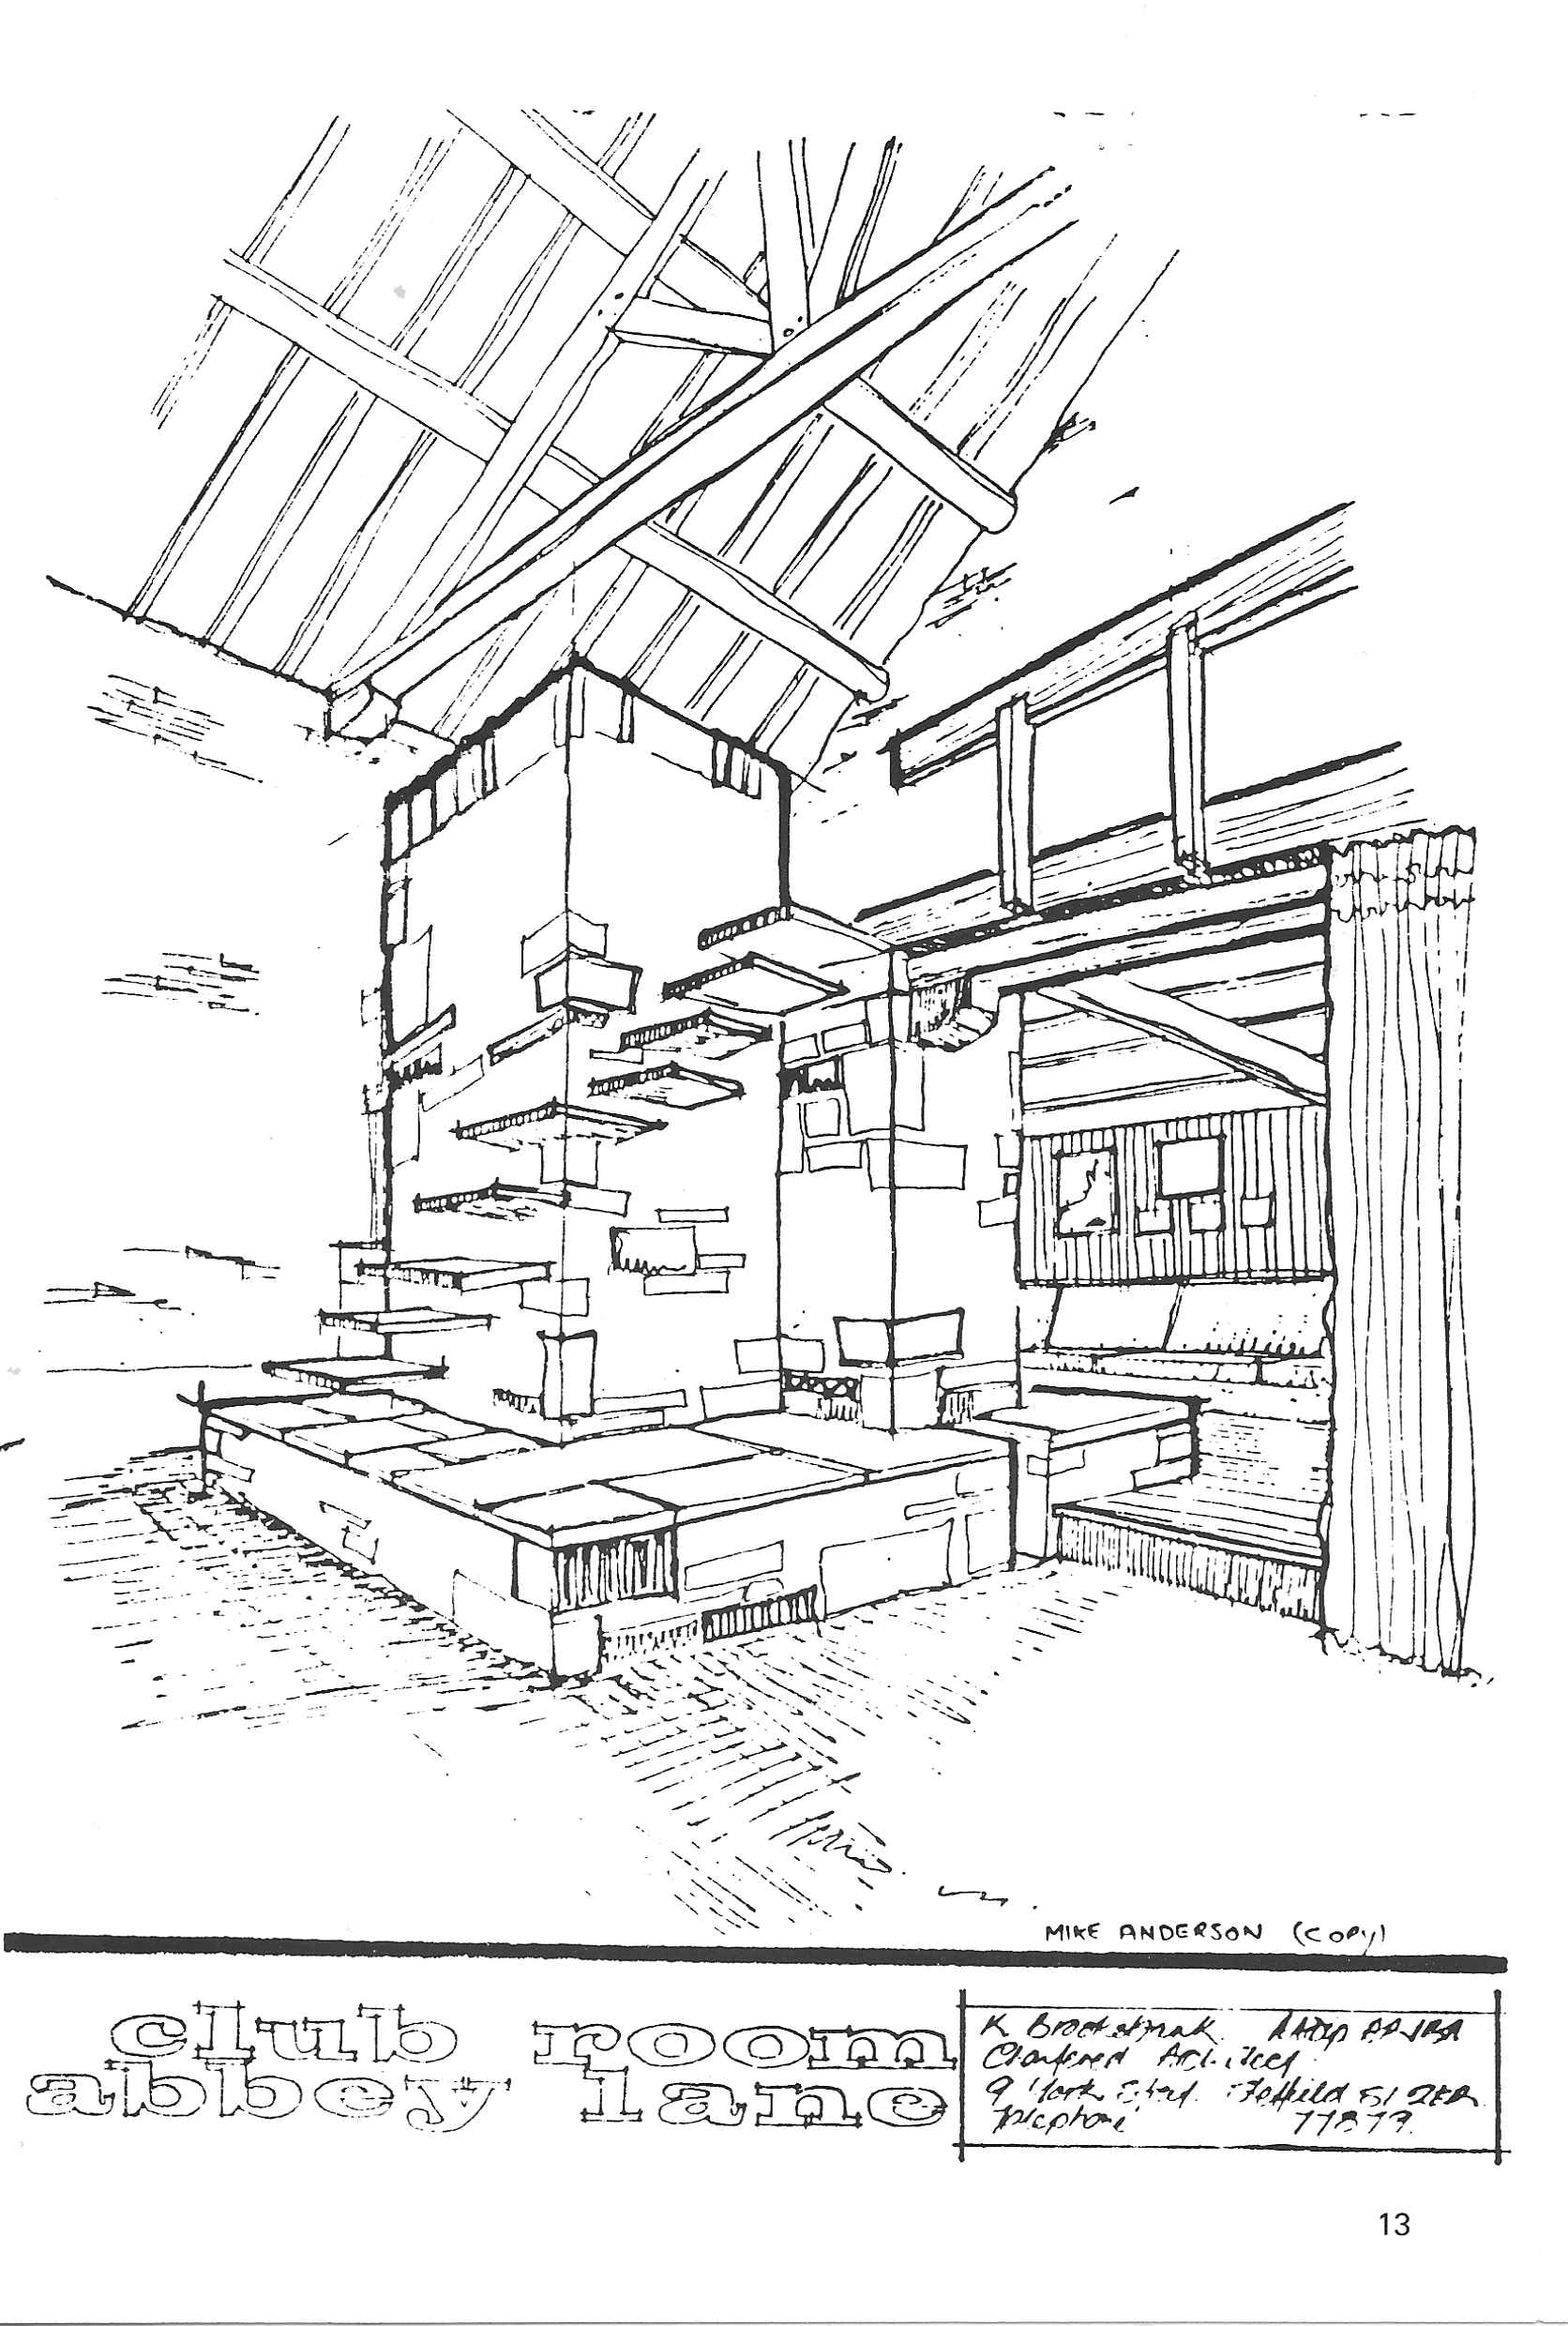
\includegraphics[width=.9\linewidth]{Plan1.jpg}
\caption{\label{fig:orgparagraph1}
The Clubroom and Climbing Wall.}
\end{figure}

\begin{figure}[htb]
\centering
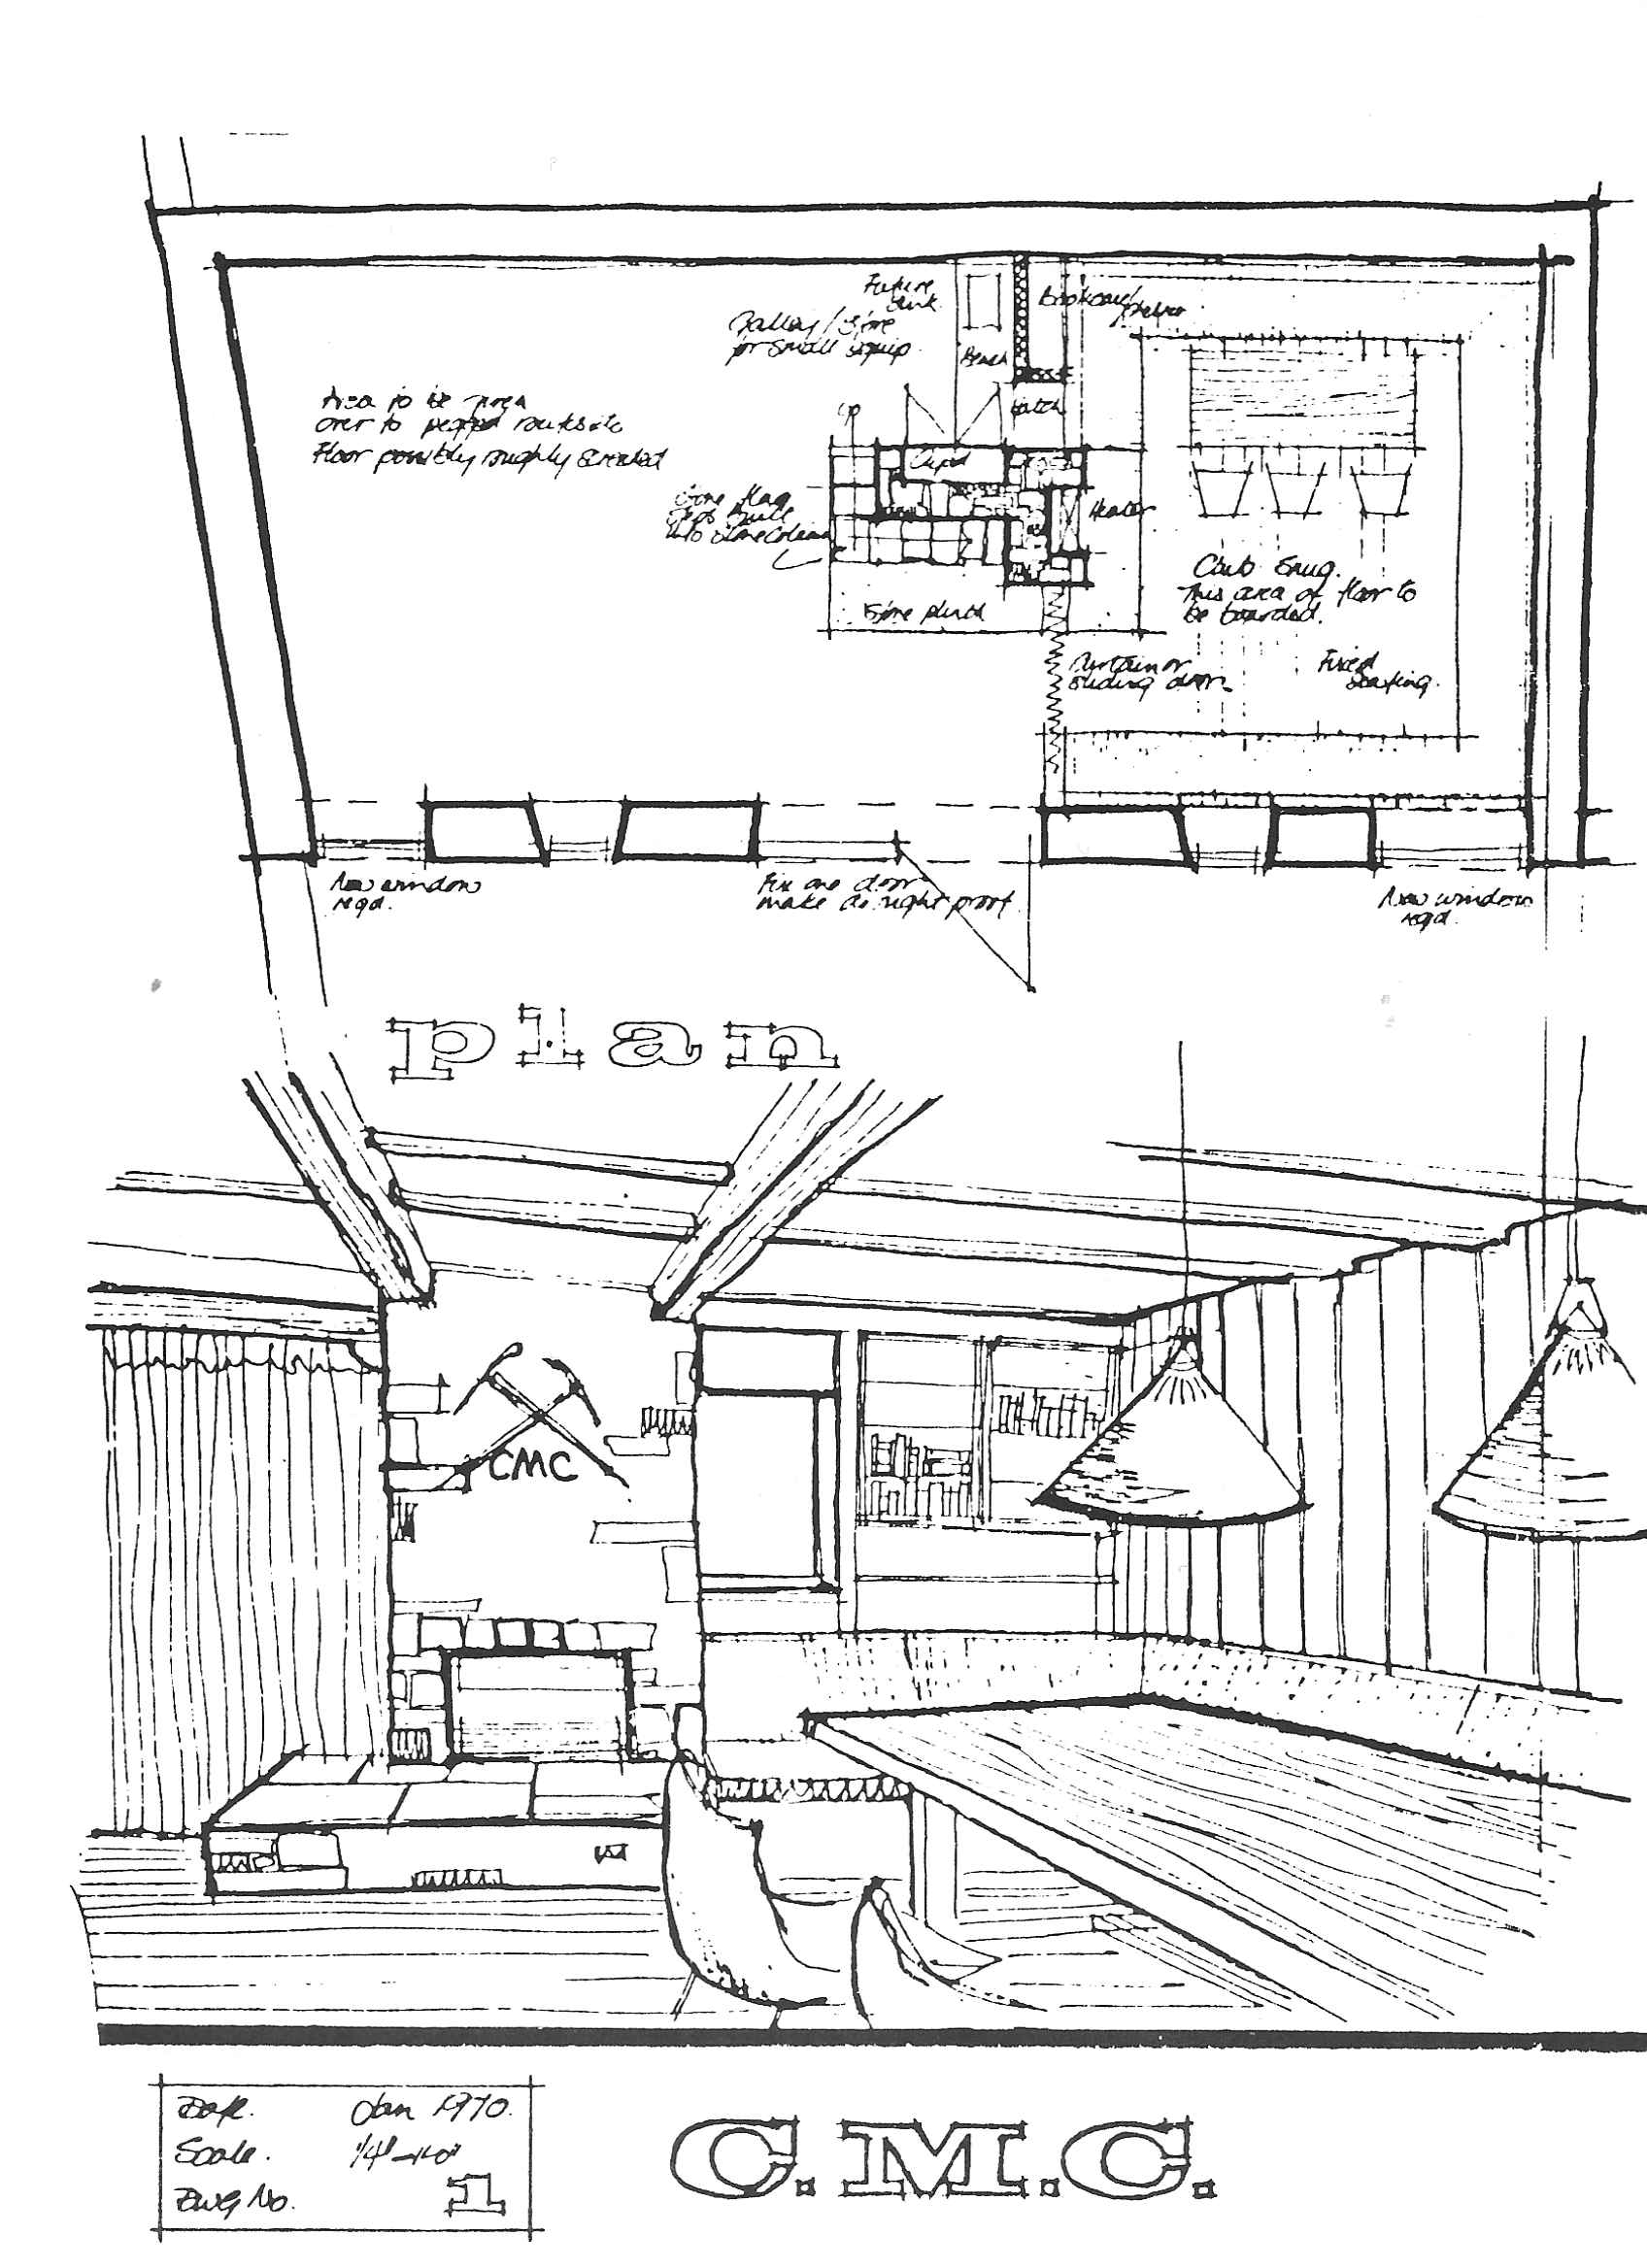
\includegraphics[width=.9\linewidth]{Plan2.jpg}
\caption{\label{fig:orgparagraph2}
The Clubroom.}
\end{figure}

\begin{figure}[htb]
\centering
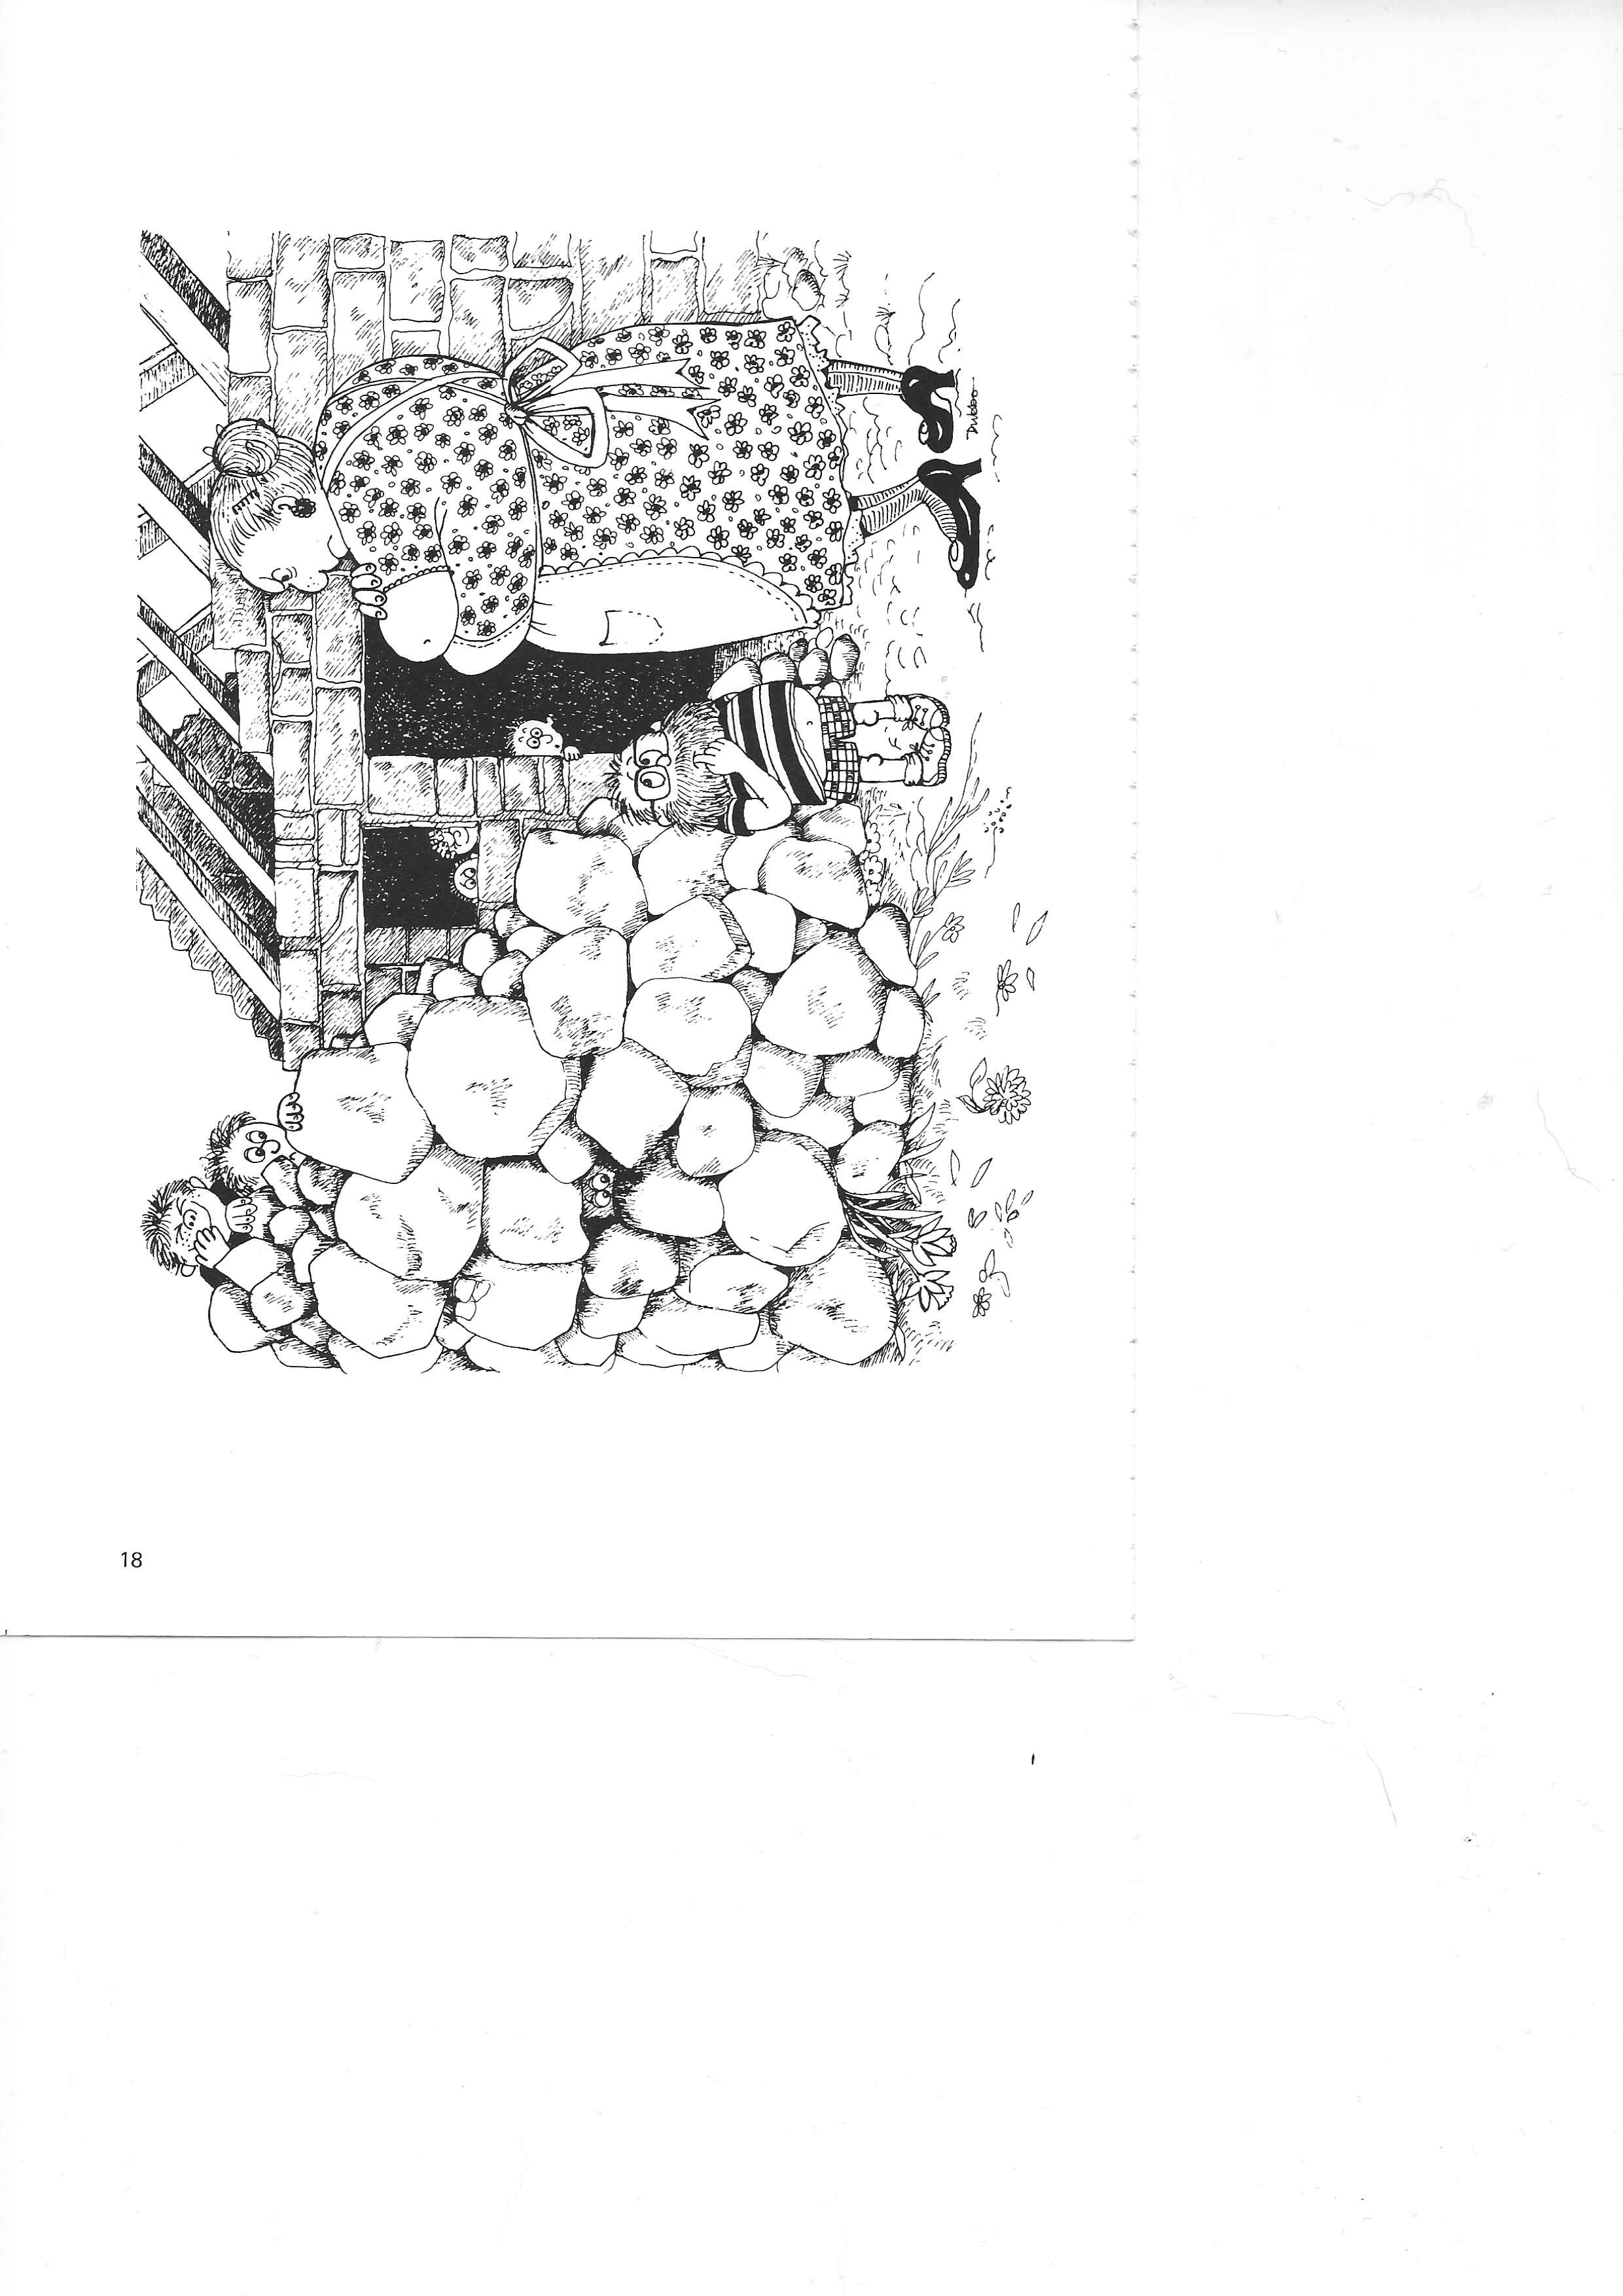
\includegraphics[width=.9\linewidth]{Cartoon_1.jpg}
\caption{\label{fig:orgparagraph3}
Renovating the Clubroom.}
\end{figure}

\chapter{Cairngorm Plateau Traverse}
\label{sec:orgheadline3}
\chapterauthor{by Mike Jackson}

\begin{figure}[htb]
\centering
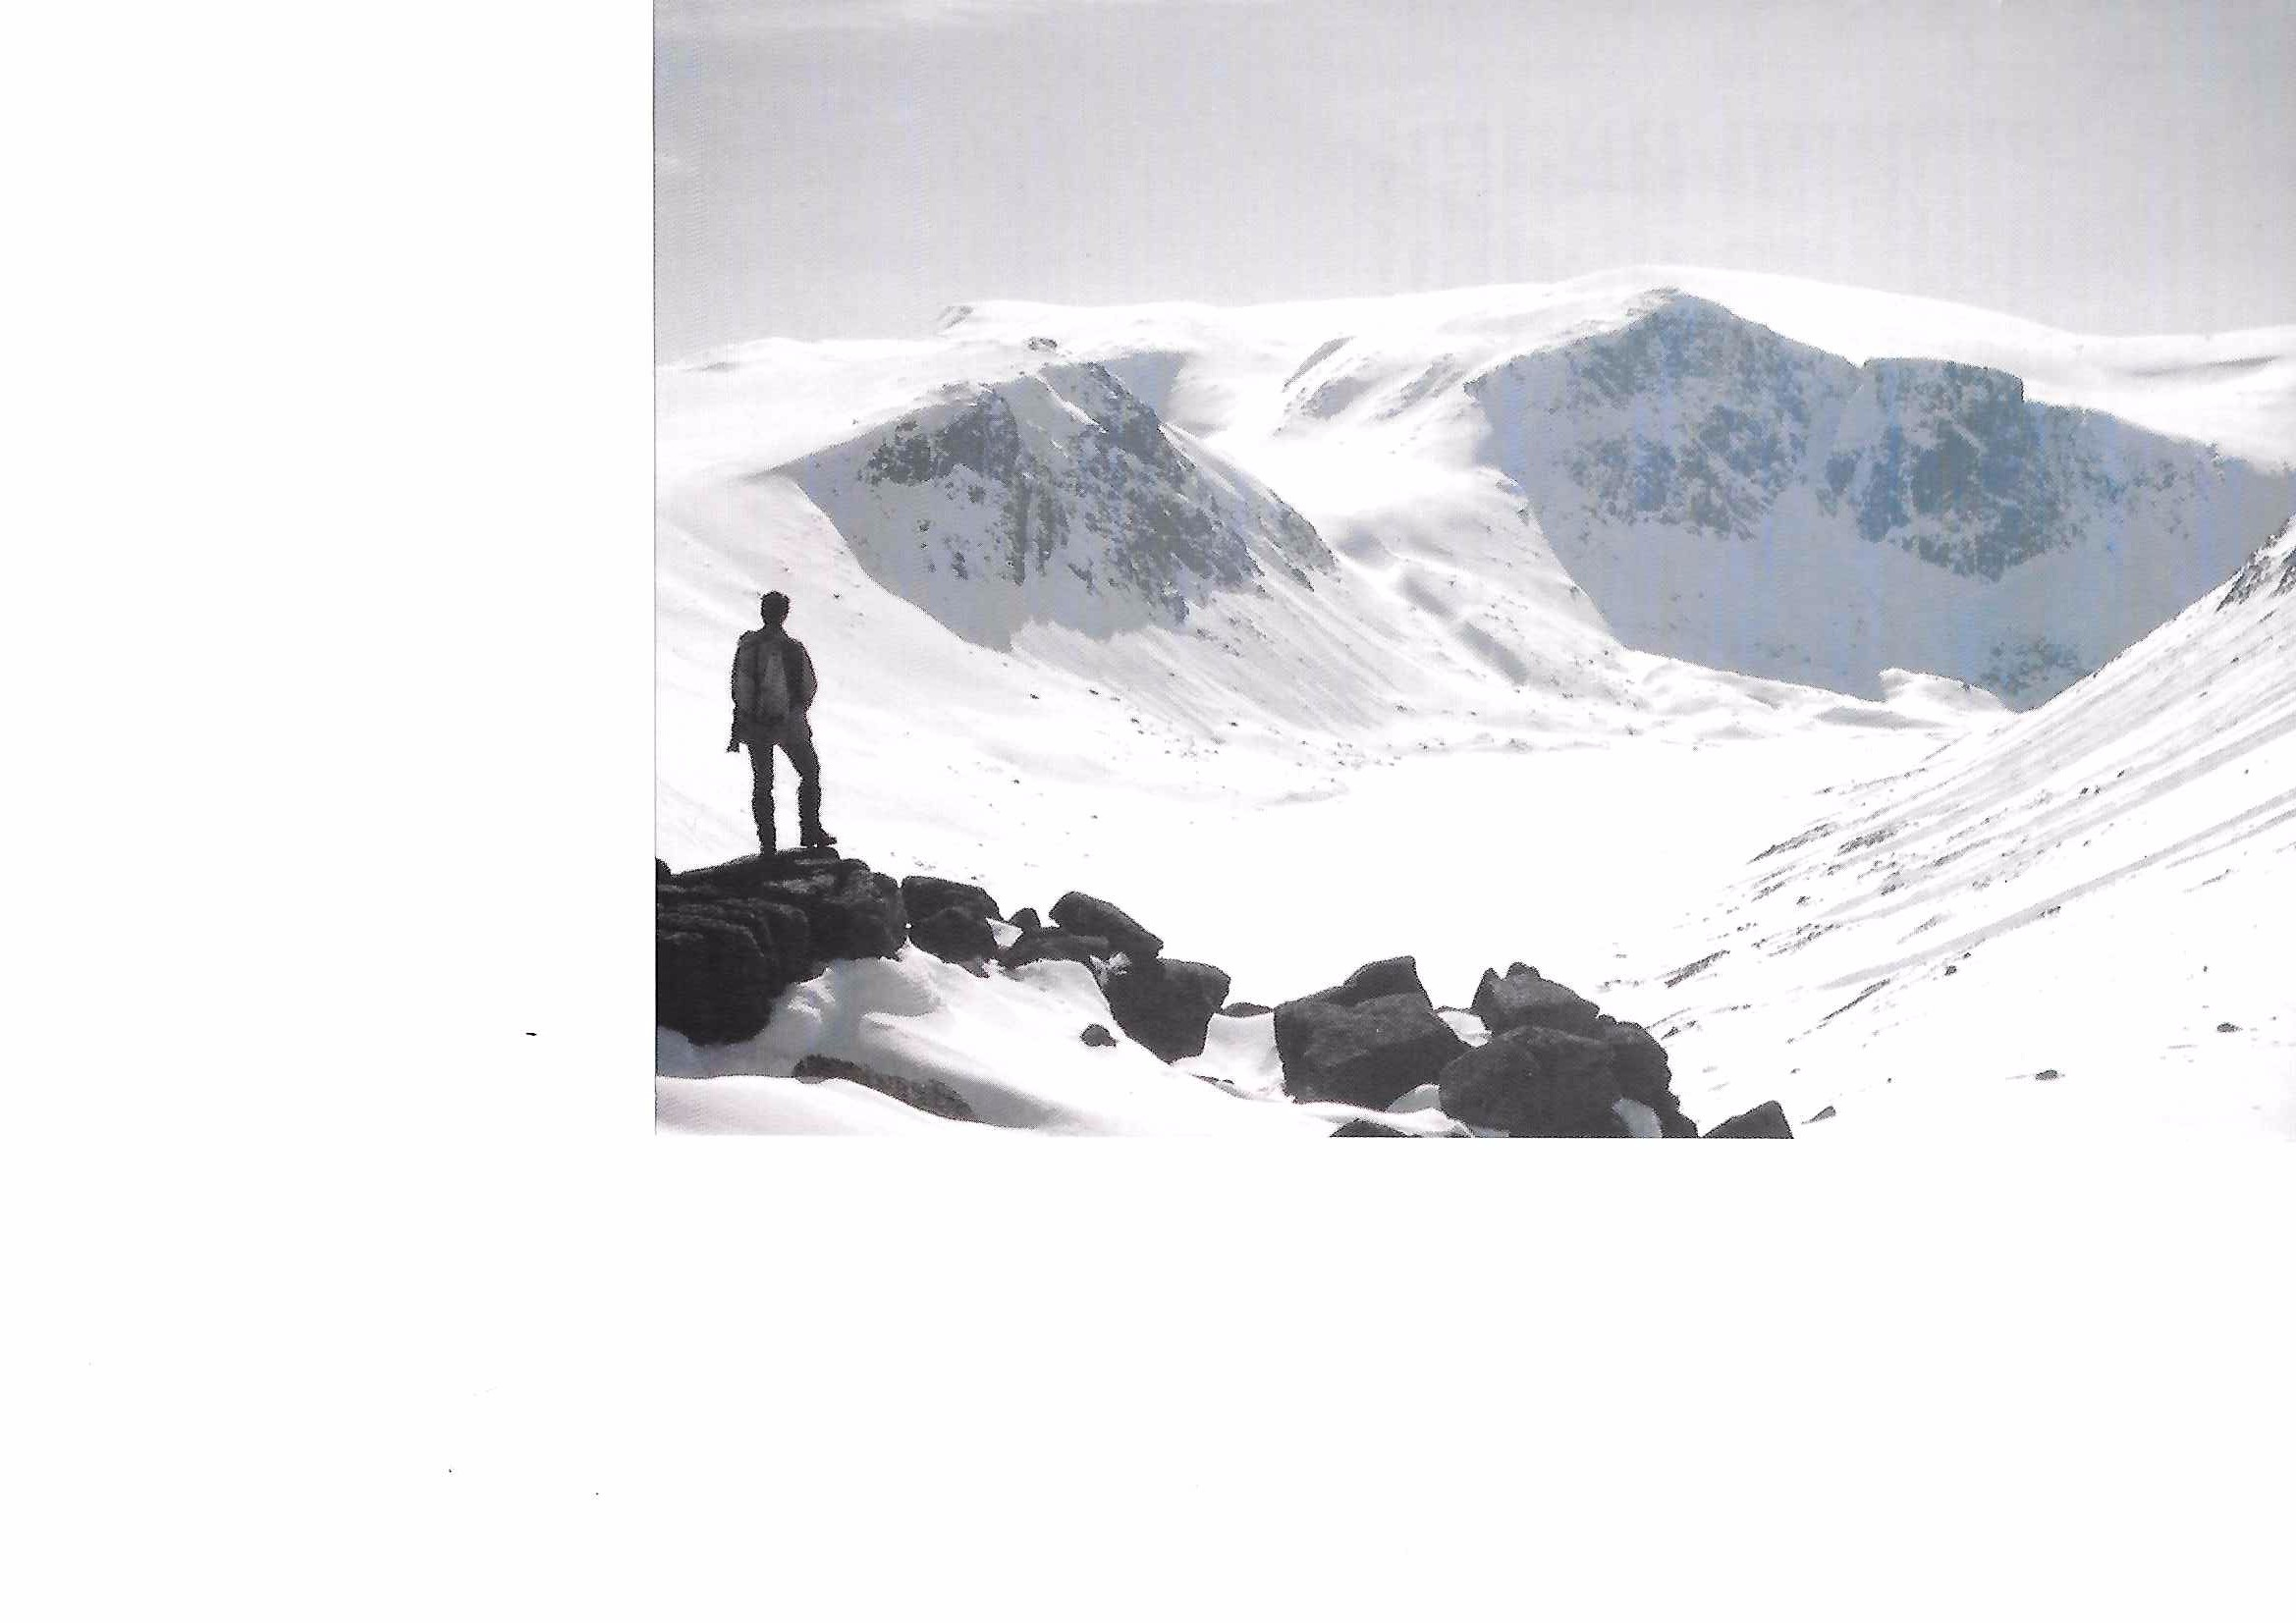
\includegraphics[width=.9\linewidth]{Ben_Macdui.jpg}
\caption{\label{fig:orgparagraph4}
Ben Macdui Beyond Loch Avon (Frank Mellor)}
\end{figure}

An annual highlight in the early days of the CMC was the
winter visit to the Cairngorms. For many members this was their
first experience of the magnificent snowscapes and near arctic
conditions to be enjoyed  or endured  in Scotland during the
winter months. A particular outing on these hills in February
1970 proved to be one  of the outstanding days of an early CMC
Cairngorm Meet and at the same time illustrates very well the
conditions one may reasonably expect to meet in winter in the
Highlands. Our party consisted of Mike Anderson, Jack Ashcroft,
Chris Taylor, Paul Goodlad, Dick Arnold and myself and our
objective was to traverse the great plateau from Cairngorm to Ben
Macdui and back.

The early morning was beautifully clear under a blue sky and
with deep snow everywhere. I regret to record that certain
members were aided in varying degrees by the chairlift in their
initial ascent of Cairngorm. I myself had to endure an
uncomfortable "stitch" but the glorious views were ample
compensation. As we descended to the west from the summit, we
could pick out a column of walkers on the plateau below,
resembling a trail of ants and giving a wonderful sense of scale
to the scene. The vista ahead of Cairn Toul, Braeriach and Sgoran
Dubh Mor was particularly splendid and there was a magnificent
view across to Fiacaill Ridge and the neighbouring cliffs
plastered in brilliant white snow with huge cornices. The going
was fairly arduous as the snow was not sufficiently frozen to
take our weight and we were constantly sinking in up to our knees
and beyond. We made our way to the Corran Bothy near Feith Buidhe
 a bothy later demolished following a tragedy hereabouts when a
number of children perished in the snows  only to find it
completely covered by snowdrifts except for the yellow chimney
cowl which stuck out grotesquely from the snow. There was a
really breathtaking view across to Braeriach with its great
coires gouged out of the plateau, all completely snow covered
under a cloudless pale blue sky. The summit of Ben Macdui gave
further wonderful views, particularly across to Cairn Toul and
the peaks beyond it, down to Carn a'Mhaim and the great snow
filled trench of the Dee and far away to Beinn a'Ghlo well to the
south. The Devil's Point, a spectacular peak when seen from the
Lairig Ghru track coming in from the south, appeared far below
our elevated position as a minor protuberance in this great
winter landscape.

It was then that my personal troubles really started as I
became very ill and had to retire urgently behind snow covered
boulders. The "stitch" which had afflicted me most of the way to
Macdui suddenly became much worse and on the return journey it
was impossible for me to walk any distance without stopping for
breath. To make matters worse, the wind began to increase and
great black clouds were approaching from the north west. The
weather closed in rapidly and the spindrift, combined with
falling snow in the mist, soon created near "white out"
conditions. Before long I was reduced to walking a few yards at a
time and later on I was able to think only as far as the next
step in the deep snow. Most of the party had gone ahead but
fortunately for me, Paul and Dick stayed behind and were able to
give much needed assistance. I had never before felt so weak and
ill on any mountain trip and I was deeply and genuinely grateful
to my good friends for their assistance  without them, my
predicament would have been very serious indeed. The last small
ascent to the top of Fiacaill a'Choire Chais seemed never ending,
but we could at last descend the ridge, suddenly emerging from
the mist and snow to look down on a hive of activity on the ski
slopes below. Within a few yards the howling winds and generally
adverse conditions on the plateau had been left behind and  after
descending only a few hundred feet it was impossible to imagine
the violence of the wind and lashing snow which had made our
return so difficult. It remained only for us to stagger down to
the ski lift and safety.

 All walkers undertaking this traverse would do well to bear
in mind the remoteness of Ben Macdui  even in these days of
chairlifts on Cairngorm  and the sudden changes of weather often
experienced in these great hills. I have never forgotten the
great contrast between our glorious sunny walk to Ben Macdui in
such wonderfully clear conditions and that return journey on
which my personal discomforts and the adverse weather conditions
combined to create a real nightmare. The views we had enjoyed
throughout the morning of these great snow covered mountains had
been outstanding under a clear winter blue sky, but the day ended
with gales, spindrift, dense mist and snowfall   a combination of
the elements among the most difficult and dangerous we learn to
face on our beautiful yet challenging mountains.
\end{document}
